%\VignetteIndexEntry{An Introduction to the SparseM Package for Sparse Linear Algebra}
\documentclass{article}
\title{SparseM:  A Sparse Matrix Package for R
\thanks{This package should be considered experimental.  The
authors would welcome comments about any aspect of the package.
This document is an R vignette prepared with the aid of \texttt{Sweave},
Leisch(2002).  Support from NSF SES 99-11184 is gratefully acknowledged.}}
\author{Roger Koenker and Pin Ng}
\usepackage{/Library/Frameworks/R.framework/Resources/share/texmf/Sweave}
\begin{document}
\maketitle
\begin{abstract}
SparseM provides some basic R functionality for linear algebra with sparse matrices.
Use of the package is illustrated by a family of linear model fitting functions that
implement least squares methods for problems with sparse design matrices.  
Significant performance improvements in memory utilization and computational 
speed are possible for applications involving large sparse matrices.
\end{abstract}
\section{Introduction}

Many applications in statistics involve large sparse matrices, matrices
with a high proportion of zero entries. \ A typical example from parametric
linear regression involves longitudinal data with fixed effects:  many indicator
variables consisting of a few ones and a large number of zero elements. \ In nonparametric
regression, e.g. smoothing splines  design matices are extremely sparse often with
less than 1\% of nonzero entries. \ Conventional algorithms for linear algebra
in such situations entail exorbitant storage requirements and many wasteful
floating point operations involving zero entries.
For some specially structured problems, e.g. banded matrices,
special algorithms are available.  But recent developments in sparse linear algebra 
have produced efficient methods for handling unstructured sparsity in a remarkably
efficient way.

Exploiting these developments, the package  SparseM provides some basic
linear algebra functionality for sparse matrices stored in several standard 
formats. \ The package attempts to make the use of these methods as transparent
as possible by adhering to the method-dispatch conventions of $R$.\footnote{
The first release of the SparseM packaged used {\it S3} method-dispatch,
the current release has adopted the new {\it S4} method dispatch.
Our thanks to Brian Ripley and Kurt Hornik for advice on this aspect of the package.}
Functions are provided for:  coercion, basic unary and binary operations on matrices
and linear equation solving.

%There have been a few linear algebra packages proposed or implemented for
%sparse matrices, see Carney, Heroux, Li, and Wu (1994), Saad (1994), Remington
%and Pozo (1996), Duff, Marrone, Radicati and Vittoli (1997), and Bank and
%Douglas (2001). 
Our implementation is based on Sparskit (Saad (1994)), which
provides one of the more complete collection of subroutines for BLAS like
functions and sparse matrix utilities available in the public domain.\footnote
{Recently, a sparse matrix version of BLAS subprograms has been
provided by Duff, Heroux and Pozo (2002). Unfortunately, it handles only
sparse matrix times dense matrix multiplication at the Level 3 Sparse BLAS,
but not sparse matrix times sparse matrix multiplication.
The sparse matrix utilities
available in Sparskit, e.g.\ masking, sorting, permuting, extracting, 
and filtering, which are not available in Sparse BLAS, are also extrememly valuable.
Sparse linear algebra is a rapidly developing field in numerical analysis and we
would expect to see many important new developments that could be incorportated into
SparseM and related code in the near future.}
Our Cholesky factorization and backsolve routines are based on Ng and Peyton
(1993), which still appears to represent the state of the art for solving linear
systems involving symmetric positive definite matrices.\footnote{There are also several new direct methods for
solving unsymmetric sparse systems of linear equations over the last decade. 
A rather comprehensive comparison of performance of some prominent
software packages for solving general sparse systems can be found in
Gupta (2002).  Unfortunately, the comparisons do not include the Peyton
and Ng algorithm employed here.
The top performer reported in the study is WSMP (Gupta, 2000)
which requires proprietary XLF Fortran complier, XLC C compilier
and the AIX operating system, and the library is not released under
the GPL license. The runner up reported
is MUMPS (Amestoy, Duff, L'Excellent and Koster, 2002) which has a 
non-commerical license but is written in Fortran 90. 
The third best performer is UMFPACK (Davis, 2002), 
which is implemented in MATLAB Version 6.0 and 
later, also has a non-commerical license. Since it is a general sparse solver
not written specifically for symmetric positive definite systems of linear
equations, it would be interesting to see how it compares with the 
Choleski factorization of Peyton and Ng adopted here.}


In Section 2 we discuss in more  detail the components of the package, provide some
examples on their use and explain the basic design philosopy. 
Section 3 discusses some refinements proposed for future implementations.

SparseM can be obtained from the Comprehensive  R Archive Network, CRAN, at
\texttt{http://cran.r-project.org/}. 

\section{Design Philosophy}

In this section we briefly describe some aspects of our design philosophy 
beginning with the question of storage modes.

\subsection{Storage Modes}

There are currently more than twenty different storage formats 
used for sparse matrices. \ Each of these formats is designed to exploit
particular features of the matrices that arise in various
applications areas to gain efficiency in both memory utilization and computation.
\ Duff, Erisman and Reid (1986) and Saad (1994) provide detailed
accounts of the various storage schemes. \ Following Saad (1994) we have
chosen compressed sparse row (\textbf{csr}) format as the primary storage mode for
SparseM.\footnote{Other sparse storage formats supported in SparseM include
compressed sparse column (\textbf{csc}), symmetric sparse row (\textbf{ssr}) and
symmetric sparse column (\textbf{ssc}). \ The data structure of \textbf{csc}
format is the same as that of \textbf{csr} format except the information is
stored column-wise. \ The\ \textbf{ssr} and \textbf{ssc} formats are special cases of
\textbf{csr} and \textbf{csc}, respectively, for symmetric matrices, 
only the information in the lower triangle is stored. 
\ We have created new class objects, \texttt{matrix.csr}, \texttt{matrix.csc},
\texttt{matrix.ssr}, \texttt{matrix.ssc}, for each of these four formats.}
\ An $n$ by $m$ matrix $A$ with real elements $a_{ij}$, stored in
\textbf{csr} format consists of three arrays:

\begin{itemize}
\item \texttt{ra}: a real array of $nnz$ elements containing the non-zero
elements of $A$, stored in row order. Thus, if $i<j$, all elements of row $i$
precede elements from row $j$. The order of elements within the rows is immaterial.

\item \texttt{ja}: an integer array of $nnz$ elements containing the column
indices of the elements stored in \texttt{ra}.

\item \texttt{ia}: an integer array of $n+1$ elements containing pointers to
the beginning of each row in the arrays \texttt{ra} and \texttt{ja}. Thus
\texttt{ia[i]} indicates the position in the arrays \texttt{ra} and
\texttt{ja} where the $i$th row begins. The last $(n+1)$st element of
\texttt{ia} indicates where the $n+1$ row would start, if it existed.
\end{itemize}

The following commands illustrate typical coercion operations.

\begin{Schunk}
\begin{Sinput}
> library(SparseM)
\end{Sinput}
\begin{Soutput}
[1] "SparseM library loaded"
\end{Soutput}
\begin{Sinput}
> a <- rnorm(5 * 4)
> a[abs(a) < 0.7] <- 0
> A <- matrix(a, 5, 4)
> A
\end{Sinput}
\begin{Soutput}
     [,1]       [,2]      [,3]       [,4]
[1,]    0 -1.2520927 0.0000000  0.0000000
[2,]    0  0.8256068 0.0000000  1.0553557
[3,]    0  2.7278160 0.0000000 -0.9552583
[4,]    0 -1.1450069 0.7368707 -0.9915961
[5,]    0  0.0000000 0.0000000  1.9204870
\end{Soutput}
\begin{Sinput}
> A.csr <- as.matrix.csr(A)
> A.csr
\end{Sinput}
\begin{Soutput}
An object of class "matrix.csr"
Slot "ra":
[1] -1.2520927  0.8256068  1.0553557  2.7278160 -0.9552583 -1.1450069  0.7368707
[8] -0.9915961  1.9204870

Slot "ja":
[1] 2 2 4 2 4 2 3 4 4

Slot "ia":
[1]  1  2  4  6  9 10

Slot "dimension":
[1] 5 4
\end{Soutput}
\begin{Sinput}
> as.matrix(A.csr)
\end{Sinput}
\begin{Soutput}
     [,1]       [,2]      [,3]       [,4]
[1,]    0 -1.2520927 0.0000000  0.0000000
[2,]    0  0.8256068 0.0000000  1.0553557
[3,]    0  2.7278160 0.0000000 -0.9552583
[4,]    0 -1.1450069 0.7368707 -0.9915961
[5,]    0  0.0000000 0.0000000  1.9204870
\end{Soutput}
\end{Schunk}
To facilitate testing we have included \texttt{read.matrix.hb} 
and \texttt{write.matrix.hb} to deal with matrices
in the Harwell-Boeing storage format.  \ A list of sites with
extensive collections of sparse matrices  in this format can be found at
\texttt{http://math.nist.gov/MatrixMarket/}. \ Details on the Harwell-Boeing format can
be found in the help files for \texttt{read.matrix.hb} and \texttt{write.matrix.hb} as well
as in the User's Guide for Harwell-Boeing Sparse Matrix Collection at
\texttt{ftp://ftp.cerfacs.fr/pub/harwell\_boeing/}.

\subsection{Visualization}
The \texttt{image} function allows users to explore the
structure of the sparsity in matrices stored in \textbf{csr} format.
In the next example we illustrate the design matrix for a bivariate
spline smoothing problem illustrated in Koenker and Mizera (2002).  The
upper 100 rows of the matrix are an identity matrix, the lower 275 rows
represent the penalty component of the design matrix.  In this example $X$
has 1200 nonzero entries, roughly 3.2 percent of the number of floating
point numbers needed to represent the matrix in dense form.  The $X'X$ form
of the matrix has 1162 nonzero elements or  11.62 percent of the entries
in the full matrix.  

\begin{center}
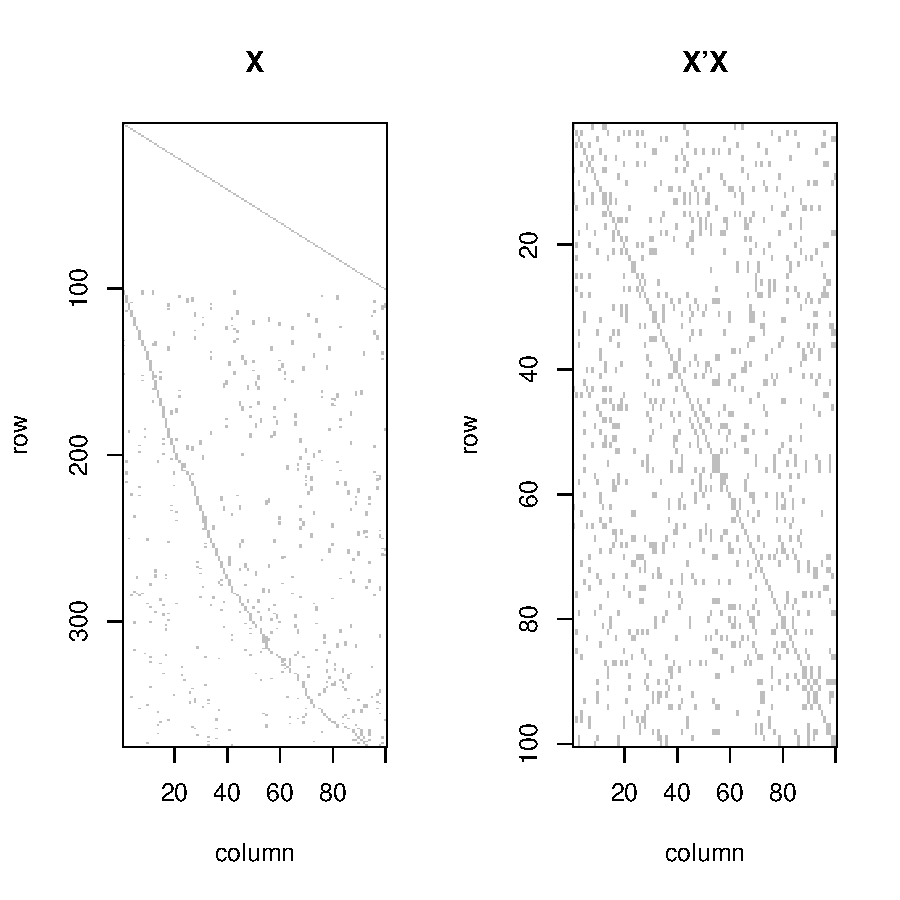
\includegraphics{SparseM-002}
\end{center}

\subsection{Indexing and Binding}

Indexing and the functions \texttt{cbind} and \texttt{rbind} for the
\texttt{matrix.csr} class work just like they do on dense matrices. 
Objects returned by \texttt{cbind} and \texttt{rbind} operating 
on objects of the \texttt{matrix.csr} class retain their 
\texttt{matrix.csr} class attribute.

\subsection{Linear Algebra}

SparseM provides a reasonably complete set of commonly used linear algebra operations for the 
\texttt{matrix.csr} class. \ The general design philosophy for 
this set of functions is that 
operations on \texttt{matrix.csr} class will yield an object also in
\texttt{matrix.csr} class with a few exceptions mentioned below.

The functions \texttt{t}, and \texttt{\%*\%} for
transposition, and multiplication of \textbf{csr} matrices work just like
their dense matrix counterparts and the returned objects retain their
\texttt{matrix.csr} class. The \texttt{diag} and \texttt{diag<-} 
functions for extracting and assigning the diagonal elements of
\textbf{csr} matrices also work like their dense matrix counterparts except
that the returned objects from \texttt{diag} are dense vectors with appropriate
zeros reintroduced.  The unary and binary functions in the group generic functions
\textsc{Ops} return objects of \texttt{matrix.csr} class.

\subsection{Linear Equation Solving} 
Research on solutions to sparse symmetric positive definite
systems of linear equations has focused primarily
on methods based on the Cholesky factorization, and we have followed this approach.
There are three functions \texttt{chol},
\texttt{backsolve} and \texttt{solve }to handle a symmetric positive definite
system of linear equations. \texttt{chol} performs Cholesky factorization
using the block sparse Cholesky algorithms of Ng and Peyton (1993). \ The
result can then be passed on to \texttt{backsolve} with a right-hand-side to
obtain the solutions. \ For systems of linear equations that only vary on the
right-hand-side, the result from \texttt{chol} can be reused,  saving
considerable computing time. \ The function \texttt{solve}, which
combines the use of \texttt{chol} and \texttt{backsolve}, 
will compute the inverse of a
matrix by default,  if the right-hand-side is missing.%
The data structure of the \texttt{chol.matrix.csr} object
produced by the sparse Cholesky method is comewhat complicated.
Users interested in recovering the Cholesky factor in some more
conventional form should recognize that the original matrix has
undergone a permutation of its rows and columns before Cholesky
factorization;  this permutation is given by the \texttt{perm}
component of the structure.  Currently no coercion methods are
supplied for the class \texttt{chol.matrix.csr}, but the
computation of the determinant by extracting the diagonal of
the Cholesky factor offers some clues for how such coercion
could be done.  This determinant is provided as a component
of the \texttt{chol.matrix.csr} structure because it can be
of some value in certain maximum likelihood applications.

\subsection{Least Squares Problems}

To illustrate the functionality of the package we include an application to
least squares regression. The group of functions \texttt{slm}, \texttt{slm.fit},
\texttt{slm.fit.csr}, \texttt{summary.slm} and \texttt{print.summary.slm} provide
analogues of the familiar \texttt{lm} family. In the current implementation
\texttt{slm} processes a formula object in essentially the same way as 
\texttt{lm}, and
calls an intermediate function \texttt{slm.fit}, which in turn calls
\texttt{slm.fit.csr} where the actual fitting occurs. Rather than the usual QR
decomposition, \texttt{slm.fit.csr} proceeds by backsolving the triangular
system resulting from a Cholesky decomposition of the $X'X$ matrix. The
sparsity of the resulting structure is usually well preserved by this
strategy. The use of sparse methods is quite transparent in the present 
\texttt{slm} implementation and \texttt{summary.slm} with the associated
\texttt{print.summary.slm} should produce identical output to their cousins in
the \texttt{lm} family. However, the speed and memory utilization can be quite
drammatically improved.  In the following problem, which involves a design
matrix that is 1850 by 712 there is a nearly three hundred fold improvement 
in speed (on a Sun Ultra 2) when we compare 
\texttt{lm.fit} and \texttt{slm.fit}.  The  comparison
is somewhat less compelling between \texttt{lm} and \texttt{slm} since 
there is a substantial common fixed cost to the setup of the problems.
In addition to the computational time saved there is also a significant
reduction in the memory required for large sparse problems.  In extreme
cases memory becomes a binding constraint on the feasibility of large
problems and sparse storage is critical in expanding the range of
problem sizes.  This is particularly true of applications in smoothing
and related image processing contexts.

\begin{Schunk}
\begin{Sinput}
> data(lsq)
> X <- model.matrix(lsq)
> y <- model.response(lsq)
> X1 <- as.matrix(X)
> slm.time <- unix.time(slm.o <- slm(y ~ X1 - 1))
> lm.time <- unix.time(lm.o <- lm(y ~ X1 - 1))
> slm.fit.time <- unix.time(slm.fit(X, y))
> lm.fit.time <- unix.time(lm.fit(X1, y))
> cat("slm time =", slm.time, "\n")
\end{Sinput}
\begin{Soutput}
slm time = 1.63 0.94 2.57 0 0 
\end{Soutput}
\begin{Sinput}
> cat("lm time =", lm.time, "\n")
\end{Sinput}
\begin{Soutput}
lm time = 3.39 1.06 4.44 0 0 
\end{Soutput}
\begin{Sinput}
> cat("slm.fit time =", slm.fit.time, "\n")
\end{Sinput}
\begin{Soutput}
slm.fit time = 0.17 0.05 0.21 0 0 
\end{Soutput}
\begin{Sinput}
> cat("lm.fit time =", lm.fit.time, "\n")
\end{Sinput}
\begin{Soutput}
lm.fit time = 2.42 0.27 2.7 0 0 
\end{Soutput}
\begin{Sinput}
> cat("slm Results: Reported Coefficients Truncated to 5  ", "\n")
\end{Sinput}
\begin{Soutput}
slm Results: Reported Coefficients Truncated to 5   
\end{Soutput}
\begin{Sinput}
> sum.slm <- summary(slm.o)
> sum.slm$coef <- sum.slm$coef[1:5, ]
> sum.slm
\end{Sinput}
\begin{Soutput}
Call:
slm(formula = y ~ X1 - 1)

Residuals:
     Min       1Q   Median       3Q      Max 
-0.19522 -0.01400  0.00000  0.01442  0.17833 

Coefficients:
     Estimate Std. Error t value Pr(>|t|)    
[1,] 823.3613     0.1274  6460.4   <2e-16 ***
[2,] 340.1156     0.1711  1987.3   <2e-16 ***
[3,] 472.9760     0.1379  3429.6   <2e-16 ***
[4,] 349.3175     0.1743  2004.0   <2e-16 ***
[5,] 187.5595     0.2100   893.3   <2e-16 ***
---
Signif. codes:  0 `***' 0.001 `**' 0.01 `*' 0.05 `.' 0.1 ` ' 1 

Residual standard error: 0.03789 on 1138 degrees of freedom
Multiple R-Squared:     1,	Adjusted R-squared:     1 
F-statistic: 4.504e+07 on 712 and 1138 DF,	p-value:     0 
\end{Soutput}
\begin{Sinput}
> cat("lm Results: Reported Coefficients Truncated to 5  ", "\n")
\end{Sinput}
\begin{Soutput}
lm Results: Reported Coefficients Truncated to 5   
\end{Soutput}
\begin{Sinput}
> sum.lm <- summary(lm.o)
> sum.lm$coefficients <- sum.lm$coefficients[1:5, ]
> sum.lm
\end{Sinput}
\begin{Soutput}
Call:
lm(formula = y ~ X1 - 1)

Residuals:
       Min         1Q     Median         3Q        Max 
-1.952e-01 -1.400e-02  1.859e-19  1.442e-02  1.783e-01 

Coefficients:
    Estimate Std. Error t value Pr(>|t|)    
X11 823.3613     0.1274  6460.4   <2e-16 ***
X12 340.1156     0.1711  1987.3   <2e-16 ***
X13 472.9760     0.1379  3429.6   <2e-16 ***
X14 349.3175     0.1743  2004.0   <2e-16 ***
X15 187.5595     0.2100   893.3   <2e-16 ***
---
Signif. codes:  0 `***' 0.001 `**' 0.01 `*' 0.05 `.' 0.1 ` ' 1 

Residual standard error: 0.03789 on 1138 degrees of freedom
Multiple R-Squared:     1,	Adjusted R-squared:     1 
F-statistic: 4.504e+07 on 712 and 1138 DF,  p-value: < 2.2e-16 
\end{Soutput}
\end{Schunk}


\section{Some Potential Refinements}

There are still many features that could be usefully added to the package. Among these
we would especially like to see: \texttt{crossprod},
\texttt{row},\texttt{ col}, code for \texttt{eigen}, \texttt{svd}
would also be desirable, but seems somewhat more problematic.
Support for other storage formats might
be eventually useful, although \textbf{csr, csc, ssr, ssc} formats seem quite
sufficient for most purposes. A major improvement in the \texttt{slm}
implementation would be to replace the line
\begin{verbatim}
X <- as.matrix.csr(model.matrix(Terms, m, contrasts))
\end{verbatim}
which coerces the dense form of the regression design matrix produced by
model.matrix into the sparse form. Ideally, this would be done with a special 
\texttt{.csr} form of
\texttt{model.matrix}, thus obviating the need to construct the dense form
of the matrix. We have not looked carefully at the question of implementing
this suggestion, but we (still) hope that someone else might be inspired to do so.

Our primary motivation for $R$ sparse linear algebra comes from
our experience, see  e.g. Koenker, Ng and Portnoy (1994) and He and Ng (1999),
with interior point algorithms for quantile regression  smoothing problems.  
We plan to report on this experience elsewhere.


\begin{center}
{\Large{\bf References}}
\end{center}

%\textsc{Bank, R.E. and  C.C. Douglas.} (1993). Sparse matrix multiplication
%package (SMMP). \textit{Advances in Computational Mathematics, 1, 127-137.}

%\textsc{Carney, Sandra, Michael A. Heroux, Guangye Li, and Kesheng Wu.}
%(1994). A revised proposal for a sparse BLAS toolkit. Technical Report 94-034,
%Army High Performance Computing Research Center.

\textsc{Amestoy, P. R., I. S. Duff, J. -Y. L'Excellent {\small and} J. Koster.} (2002).
MUltifrontal Massively Parallel Solver (MUMPS Version 4.2 beta) Users' Guide,
http://www.enseeiht.fr/lima/apo/MUMPS/

\textsc{Davis, T. A.} (2002). UMFPACK Version 4.0 User Guide,
\newline
http://www.cise.ufl.edu/research/sparse/umfpack.

\textsc{Duff, I.S., A. M. Erisman {\small and} J. K. Reid.} (1986). \textit{Direct
Methods for Sparse Matrices}, Clarendon Press, Oxford.

\textsc{Duff, I. S., M. A. Heroux, {\small and} R. Pozo.} (2002).
``An Overview of the Sparse Basic Linear Algebra Subroutines: The
New Standard from the BLAS Technical Forum,'' \emph{ACM Transactions
on Mathematical Software}, 28, 239-267.

%\textsc{Duff, I. S., M. Marrone, G. Radicati, and C. Vittoli.} (1997). Level 3
%Basic Linear Algebra Subprograms for sparse matrices: a user level interface.
%\textit{ACM Trans. Math. Softw}., 23(3):379--401.

\textsc{Gupta, A.} (2000). WSMP: Watson Sparse Matrix Package (Part-II:
direct solution of general sparse systems). Technical Report RC 21888 (98472),
IBM T.J. Watson Research Center, Yorktown Heights, N.Y., 
http://www.cs.umn.edu/
\newline
$\sim$agupta/doc/wssmp-paper.ps

\textsc{Gupta, A.} (2002). ``Recent Advances in Direct Methods for
Solving Unsymmetric Sparse Systems of Linear Equations,'' \emph{ACM 
Transactions on Mathematical Software}, 28, 301-324.

\textsc{He, X.,  {\small and} P.~Ng}  (1999): ``COBS: {Q}ualitatively
  Constrained Smoothing Via Linear Programming,'' \emph{Computational
  Statistics}, 14, 315--337.

\textsc{Koenker, R., P.~Ng,  {\small and} S.~Portnoy}  (1994): ``Quantile
  smoothing splines,'' \emph{Biometrika}, 81, 673--680.

\textsc{Leisch, F.} (2002). Sweave:  Dynamic Generation of Statistical Reports
Using Literate Data Analysis, \texttt{http://www.wu-wien.ac.at/am}.

\textsc{Koenker, R. {\small and} Mizera, I} (2002). Penalized Triograms:  Total
Variation Regularization for Bivariate Smoothing, preprint.

\textsc{Ng, E. G. {\small and} B. W. Peyton}. (1993) Block sparse Cholesky algorithms
on advanced uniprocessor computers'', \textit{SIAM J. Sci. Comput.}, 
14, 1034-1056.

\textsc{Saad, Y.} (1994) Sparskit: A basic tool kit for sparse matrix
computations; Version 2, 
\texttt{http://www.cs.umn.edu/Research/arpa/SPARSKIT/sparskit.html}

\end{document}
